\section{Putting Together}
\label{sec:putting-together}

After ADU definition is given and overall namespace design determined, it's natural to come up the namespace structure by putting previous ideas together.
In this detailed namespace illustrated in Fig~\ref{fig:overall-namespace}, \textit{Effective scope} are represented with series of name components ranging from zero to two, and timestamp is appened to achieve the Data name uniqueness.

\begin{figure}[!h]
    \centering
    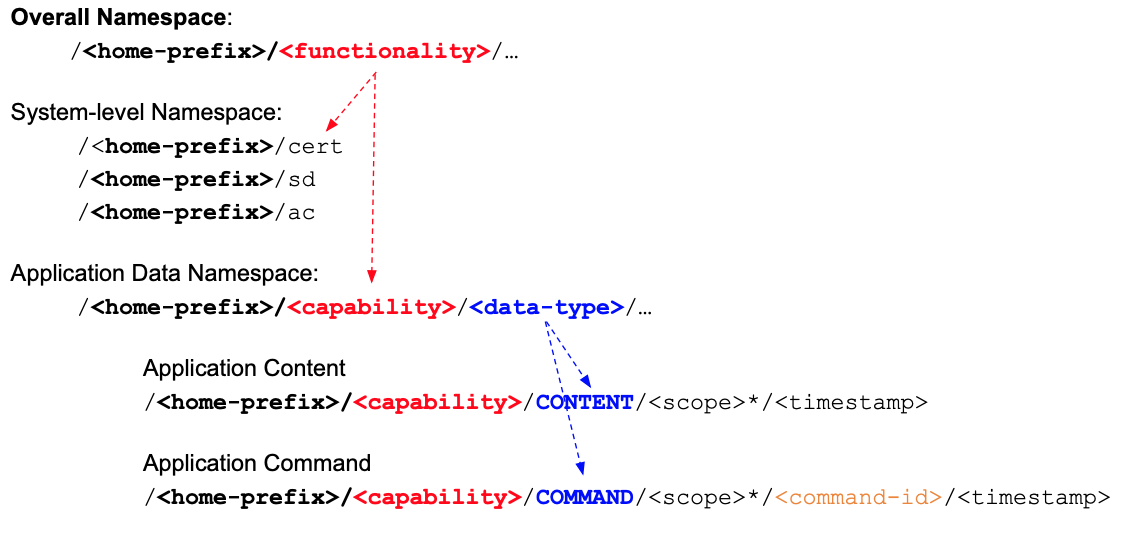
\includegraphics[width=0.5\textwidth]{overall-namespace}
    \caption{Overall NDN-Lite Namespace}
    \label{fig:overall-namespace}
\end{figure}

The last problem not solved is to name identities.
To simplify certificate and trust management, identity names are only allowed binded with one capability.
Multipurpose sensers or applications will host multiple certificates and sign packets with corresponding identities as a result.
Another factor to consider the finest granularity in data publishing.
Content type data, unlike commands often explicitly assigned to an effective scope in data production time, thus need to assign a default fine-grained scope for applications falling back.
We assign this scope in identity names during the bootstrapping time.

\begin{figure}[!h]
    \centering
    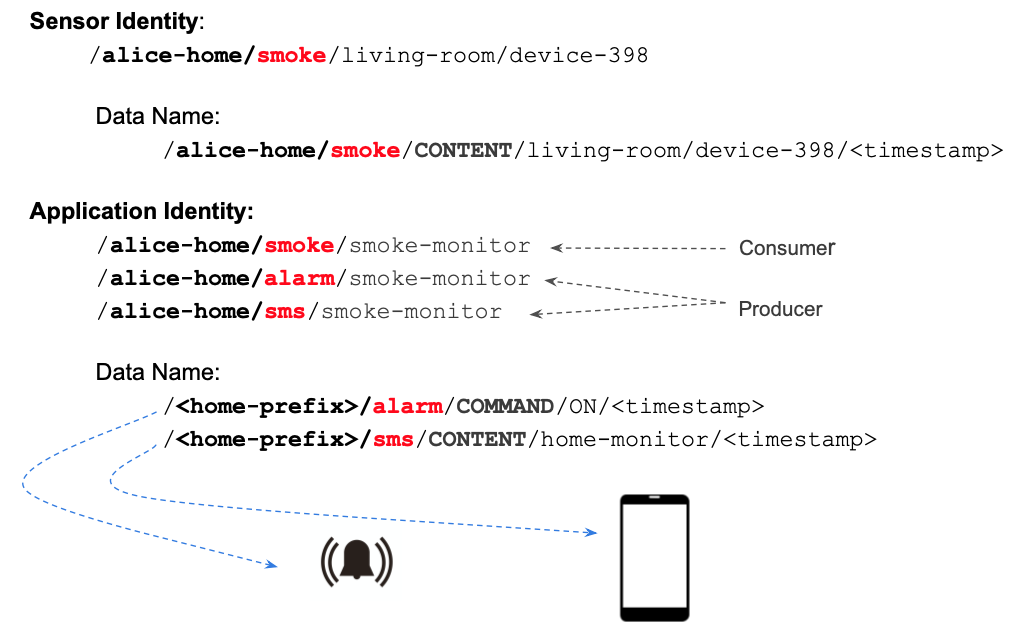
\includegraphics[width=0.5\textwidth]{case-study}
    \caption{Example Application: Smoke Monitor}
    \label{fig:case-study}
\end{figure}

The complete workflow is demonstrated by a case study in Fig~\ref{fig:case-study} with a smoke monitoring application.
Smoke detector installed in the living room is named with \textsl{/alice-home/smoke/living-room/device-398}.
Its encryption key for publishing data under prefix \textsl{/alice-home/smoke} is obtained from access controller residing in \textsl{/alice-home/ac}.
To avoid ambiguities in naming in detection data publishing, data names falls back to \textit{effective-scope} with \textsl{/living-room/device-398}.
The smoke monitor application is installed in the home hub, and three different identities are bootstrapped by this application.
Through subscribing prefix \textsl{/alice-home/smoke}, smoke monitor receive smoke detection data and perform trust schema checking and data decryption.
Its decryption key is obtained from access controller in the same way with smoke detector.
Then two data are published under \textsl{/alice-home/alarm} and \textsl{/alice-home/sms}.
Alarm command issued should be effective in the entire home since not specific \textit{effective-scope} is given.
Meanwhile, user's smartphone which subscribes \textsl{/alice-home/sms} will receive the notification.